\subsubsection{1(d)}
\textbf{\textit{Problem}}: In Figure~\ref{1_d}, N designates a plane that is made to rotate with constant angular speed $\omega$ about a line $Z$ fixed in $N$ and in a reference frame $R$. The unit vectors $\pmb n_x, \pmb n_y$ and  $\pmb n_z$ are mutually perpendicular and fixed in R, and $\pmb n$ is a unit vector normal to $N$ and equal to $\pmb n_x$ at time $t=0$. Finally, $P_1$ and $P_2$ represent particles connected to each other by a rigid rod of lenghth $L$, these particles remaining at all times in contact with $N$.

\begin{figure}[H]
    \centering
    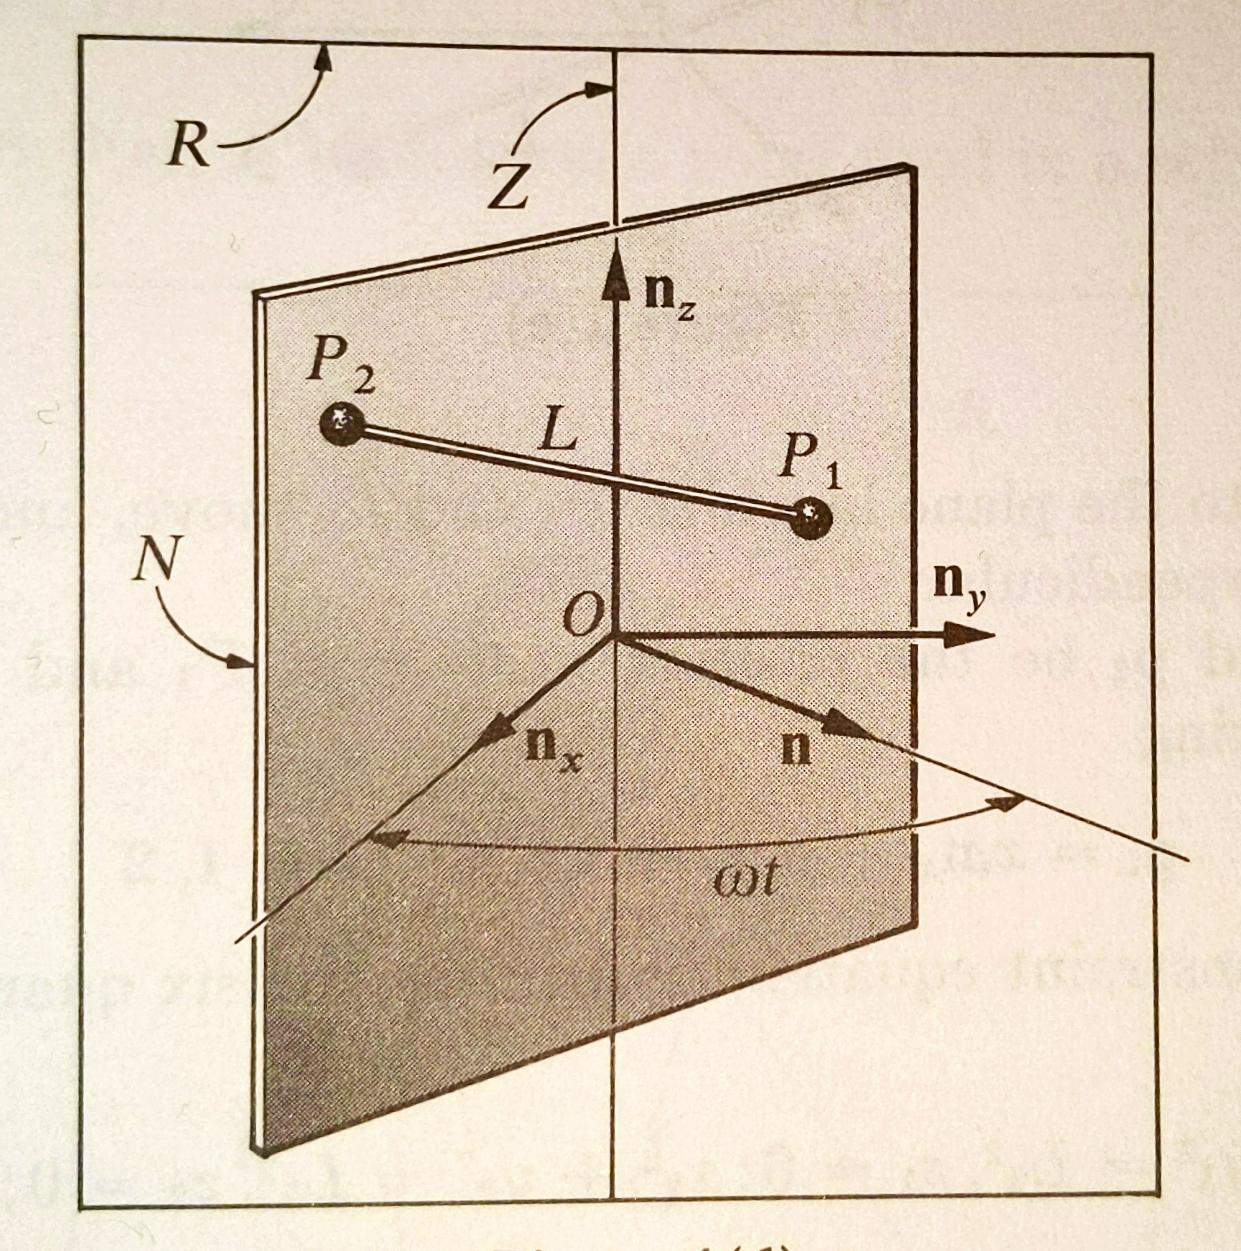
\includegraphics[width = 0.35\textwidth, height = 0.3\textwidth]{figs/ProbSet_1/1_d.jpg}
    \caption{}
    \label{1_d}
\end{figure}


Letting $\pmb p_1$ and $\pmb p_2$ be the position vectors of $P_1$ and $P_2$ relative to a point $O$ fixed in line $Z$, and taking

$$\pmb p_i = x_i \pmb n_x + y_i \pmb n_y + z_i \pmb n_z \qquad i = 1, 2$$

detarmine functions $f_j(x_1, y_1, z_1, x_2, y_2, z_2, t)$, for $j=1, 2, 3$, such that the requirements that $P_1$ and $P_2$ remain in $N$ and be separated by distance $L$ can be experessed as $f_j = 0$, $j = 1, 2, 3$.

\textbf{\textit{Sol.}}:

\begin{enumerate}
    \item For $P_1$ and $P_2$ to be attached to $N$ at all times,
    \begin{align*}
        \pmb p_i .  \pmb n &= 0 \quad \forall \; t, \qquad i = 1, 2\\
        \text{We have, } \qquad &\\
        \pmb n(t) &= \pmb n_x \sin \omega t + \pmb n_y \cos \omega t\\
        \\
        \implies \pmb p_i .  \pmb n &= x_i \sin \omega t + y_i \cos \omega t = 0 \qquad i=1, 2\\
        \\
        \therefore f_1 &= x_1 \sin \omega t + y_1 \cos \omega t\\
                   f_2 &= x_2 \sin \omega t + y_2 \cos \omega t
    \end{align*}

    \item For the distance between $P_1$ and $P_2$ to remain $L$:
    \begin{align*}
        \norm{\pmb p_1 - \pmb p_2} &= L\\
        \\
        \implies f_3 &= (x_1 - x_2)^2 + (y_1 - y_2)^2 + (z_1 - z_2)^2 - L^2
    \end{align*}
\end{enumerate}

\textbf{Note}: $f_1, f_2, f_3$ are holonomic constraints. $f_1, f_2$ are rheonomic and $f_3$ is scleronomic.\\

A \itbf{holonomic} constraint is a \itbf{kinematic constraint} equations that only involves position vectors (\itbf{scleronomic}) or can be integrated to position vectors and time (\itbf{rheonomic}) with none of it's derivatives. If a kinematic constraint equations has non-integrable derivatives of position vectors, then they are \itbf{non-holonomic} constraints.
